\documentclass{article}
\usepackage{graphicx} % Required for inserting images
\usepackage{amsmath}
\usepackage{amssymb} % used for math symbols
\usepackage{mathtools}

\makeatletter
\newcommand*{\rom}[1]{\expandafter\@slowromancap\romannumeral #1@}
\makeatother

\title{Computer Grafik Blatt 3}
\date{May 2023}

\begin{document}

\maketitle

\section*{Aufgabe 1:}

\subsection*{a)}

\subsubsection*{1.}

Da nicht anderweitig Spezifiziert, gehen wir von einem symmetrischenm Pyramidenstumpf aus.
\[
    \begin{pmatrix}
        \frac{2n}{w} & 0            & 0                & 0                \\
        0            & \frac{2n}{h} & 0                & 0                \\
        0            & 0            & \frac{-f-n}{f-n} & \frac{-2fn}{f-n} \\
        0            & 0            & -1               & 0
    \end{pmatrix}=
\]\[
    \begin{pmatrix}
        \frac{42}{2\cdot\tan(45)\cdot21} & 0                                & 0                  & 0                    \\
        0                                & \frac{42}{2\cdot\tan(30)\cdot21} & 0                  & 0                    \\
        0                                & 0                                & \frac{-6021}{5979} & \frac{-252000}{5979} \\
        0                                & 0                                & -1                 & 0
    \end{pmatrix}=
\]\[
    \begin{pmatrix}
        1 & 0        & 0                  & 0                   \\
        0 & \sqrt{3} & 0                  & 0                   \\
        0 & 0        & -\frac{2007}{1993} & -\frac{84000}{1993} \\
        0 & 0        & -1                 & 0
    \end{pmatrix}
\]

\subsubsection*{2.}
\[Punkt(Rechts-Oben-Vorne)=
    \begin{pmatrix}
        n\cdot \tan(45) \\
        n\cdot \tan(30) \\
        -n              \\
        1
    \end{pmatrix}=
    \begin{pmatrix}
        21        \\
        7\sqrt{3} \\
        -21       \\
        1
    \end{pmatrix}
\]
\[
    Punkt(Links-Unten-Hinten)=
    \begin{pmatrix}
        -f\cdot \tan(45) \\
        -f\cdot\tan(30)  \\
        -f               \\
        1
    \end{pmatrix}=
    \begin{pmatrix}
        -6000        \\
        -3464.101615 \\
        -6000        \\
        1
    \end{pmatrix}
\]
\subsubsection*{3.}
\[
    \begin{pmatrix}
        1 & 0        & 0                  & 0                   \\
        0 & \sqrt{3} & 0                  & 0                   \\
        0 & 0        & -\frac{2007}{1993} & -\frac{84000}{1993} \\
        0 & 0        & -1                 & 0
    \end{pmatrix}
    \begin{pmatrix}
        21        \\
        7\sqrt{3} \\
        -21       \\
        1
    \end{pmatrix}=
    \begin{pmatrix}
        21  \\
        21  \\
        -21 \\
        21
    \end{pmatrix}\rightarrow
    \begin{pmatrix}
        1 \\1\\-1\\1
    \end{pmatrix}=P(rov)\checkmark
\]
\[
    \begin{pmatrix}
        1 & 0        & 0                  & 0                   \\
        0 & \sqrt{3} & 0                  & 0                   \\
        0 & 0        & -\frac{2007}{1993} & -\frac{84000}{1993} \\
        0 & 0        & -1                 & 0
    \end{pmatrix}
    \begin{pmatrix}
        -6000        \\
        -3464.101615 \\
        -6000        \\
        1
    \end{pmatrix}=
    \begin{pmatrix}
        -6000 \\
        -6000 \\
        6000  \\
        6000
    \end{pmatrix}\rightarrow
    \begin{pmatrix}
        -1 \\-1\\1\\1
    \end{pmatrix}=P(luh)\checkmark
\]

\subsection*{b)}
Sei \[ P_1=
    \begin{pmatrix}
        18 \\-14
    \end{pmatrix}\]
\[ P_2=
    \begin{pmatrix}
        -3 \\4
    \end{pmatrix}\]
\[ P_3=
    \begin{pmatrix}
        11 \\-8
    \end{pmatrix}\]

Lösen der Gleichungen
\[
    \begin{aligned}
        \begin{pmatrix}
            11 \\ -8
        \end{pmatrix} & = \alpha \cdot 
        \begin{pmatrix}
            18 \\ -14
        \end{pmatrix} + \beta \cdot 
        \begin{pmatrix}
            -3 \\ 4 
        \end{pmatrix} \\
        1 & = \alpha + \beta
    \end{aligned}
\]

Ergebnis: $\alpha = \frac23, \beta = \frac13$

\subsection*{c)}
\[
    a = \begin{pmatrix}
        0 \\ 0
    \end{pmatrix},
    b = \begin{pmatrix}
        1 \\ 5
    \end{pmatrix},
    c = \begin{pmatrix}
        -4 \\ 4
    \end{pmatrix},
    p = \begin{pmatrix}
        1 \\ -7
    \end{pmatrix}
\]

\[
    \begin{aligned}
        A(\triangle_{abc}) & = \frac{1}{2} \cdot det \begin{pmatrix}
                                                         |   & |   \\
                                                         b-a & c-a \\
                                                         |   & |
                                                     \end{pmatrix}                                           \\
                           & = \frac{1}{2} \cdot det \begin{pmatrix}
                                                         1 & -4 \\
                                                         5 & 4
                                                     \end{pmatrix}                                           \\
                           & = \frac{1}{2} \cdot (1 \cdot 4 - (-4) \cdot 5) = \frac{1}{2} \cdot 24 = 12       \\
        A(\triangle_{pbc}) & = \frac{1}{2} \cdot det \begin{pmatrix}
                                                         |   & |   \\
                                                         b-p & c-p \\
                                                         |   & |
                                                     \end{pmatrix}                                           \\
                           & = \frac{1}{2} \cdot det \begin{pmatrix}
                                                         0  & -5 \\
                                                         12 & 11
                                                     \end{pmatrix}                                           \\
                           & = \frac{1}{2} \cdot (0 \cdot 11 - (-5) \cdot 12) = \frac{1}{2} \cdot 60 = 30     \\
        A(\triangle_{pca}) & = \frac{1}{2} \cdot det \begin{pmatrix}
                                                         |   & |   \\
                                                         c-p & a-p \\
                                                         |   & |
                                                     \end{pmatrix}                                           \\
                           & = \frac{1}{2} \cdot det \begin{pmatrix}
                                                         -5 & -1 \\
                                                         11 & 7
                                                     \end{pmatrix}                                           \\
                           & = \frac{1}{2} \cdot ((-5) \cdot 7 - (-1) \cdot 11) = \frac{1}{2} \cdot -24 = -12 \\
        A(\triangle_{pab}) & = \frac{1}{2} \cdot det \begin{pmatrix}
                                                         |   & |   \\
                                                         a-p & b-p \\
                                                         |   & |
                                                     \end{pmatrix}                                           \\
                           & = \frac{1}{2} \cdot det \begin{pmatrix}
                                                         -1 & 0  \\
                                                         7  & 12
                                                     \end{pmatrix}                                           \\
                           & = \frac{1}{2} \cdot ((-1) \cdot 12 - 0 \cdot 7) = \frac{1}{2} \cdot -12 = -6     \\
    \end{aligned}
\]

\[
    \begin{aligned}
        \alpha & = \frac{A(\triangle_{pbc})}{A(\triangle_{abc})} = \frac{30}{12} = \frac{5}{2}  \\
        \beta  & = \frac{A(\triangle_{pca})}{A(\triangle_{abc})} = \frac{-12}{12} = -1          \\
        \gamma & = \frac{A(\triangle_{pab})}{A(\triangle_{abc})} = \frac{-6}{12} = -\frac{1}{2} \\
    \end{aligned}
\]

\subsection*{d)}


\[
    p_1 =
   \begin{pmatrix}
   24 \\ -9
   \end{pmatrix},
   p_2 =
   \begin{pmatrix}
   27 \\ 1
   \end{pmatrix} 
\]
   \begin{center}
   Steigung $= \frac{1-(-9)}{27-24}=\frac{10}{3} > 1 \Rightarrow$ Koordinaten tauschen
   \end{center}
   
\[
    p_1' =
   \begin{pmatrix}
   -9 \\ 24
   \end{pmatrix},
   p_2' =
   \begin{pmatrix}
   1 \\ 27
   \end{pmatrix} 
\]
   \begin{center}
   Steigung $= \frac{3}{10}$\checkmark
   \end{center}

\begin{table}[]
    \centering
    \begin{tabular}{|c|c|c|c|c|c|c|c|c|c|c|c|}
         \hline
         x' & -9 & -8 & -7 & -6 & -5 & -4 & -3 & -2 & -1 & 0 & 1 \\
         \hline
         y' & 24 & $24\frac{3}{10}$ & $24\frac{6}{10}$ & $-24\frac{9}{10}$ & $25\frac{2}{10}$ & $25\frac{5}{10}$ & $25\frac{8}{10}$ & $26\frac{1}{10}$ & $26\frac{4}{10}$ & $26\frac{7}{10}$ & 27  \\
         \hline
         $\lfloor y' \rceil$ & 24 & 24 & 25 & 25 & 25 & 26 & 26 & 26 & 26 & 27 & 27\\
         \hline
    \end{tabular}
    \caption{Bresenham Koordinaten}
    \label{tab:my_label}
\end{table}

Nach rücktausch der Koordinaten ergibt sich:
\begin{center}
    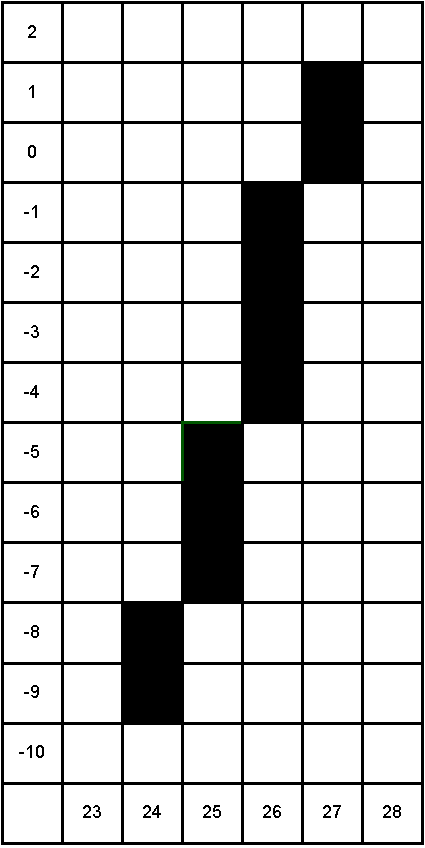
\includegraphics[width=0.5\textwidth,keepaspectratio]{KikusfuerCG.drawio.pdf}
\end{center}


\end{document}